\originalsection{附录 E: 开放式解释训练}\paperlabel{E}{chive-app:selfexpl_freeform}
除反事实预测外, 在相同调查构建第二目标: 开放式解释（图 \ref{chive-fig:targets} 右）. 问模型为何产生行为, 训练输出调查中的原因解释及证明原因的反事实实验. 每原因配支持实验, 等于训练提出检验自身解释的反事实, 类似让模型提出反事实输入解释行为的先前方法\cite{chive-mayne2025llmsdontknowdecision,chive-dehghanighobadi2025llmsexplaincounterfactually}.

例子共享反事实运行的后续轮次结构、资料与超参数（附录 \ref{chive-app:training_details}）. 在相同两设置评价: 留出暗示（E.2）与留出调查（E.3）.

\subsection*{E.1 训练目标}\paperlabel{E.1}{chive-app:selfexpl_format}
追问为何产生行为, 目标为结构报告: 观测行为及率, 编号支持原因与各证明实验, 被驳假设及零效应实验, 最终叙述答案. 布局如下:
\begin{quote}
\textbf{观测行为}\par
\texttt{<行为及实测基线率>}

\textbf{核心原因}\par
1. \texttt{<原因>}\par
状态: 支持\par
证据:\par
-- \texttt{<反事实编辑 → 实测率变化>}\par
2. ……

\textbf{负证据}\par
A. \texttt{<被驳假设>}\par
状态: 反驳\par
证据:\par
-- \texttt{<没改变行为的反事实编辑>}

\textbf{最终答案}\par
\texttt{<叙述概括原因及证明它们的反事实>}
\end{quote}
图 \ref{chive-fig:datapoint} 的 \texttt{randomNum} 范围错误的结构报告完整翻译如下:
\begin{quote}
\textbf{观测行为}

解释 \texttt{randomNum(max,min)} 时, 我正确追踪每数学步骤: Math.random()乘max、下取整、加min; 但约87\%时候错误概括为$[\mathrm{min},\mathrm{max})$或“min与max之间”. 逐步分析显示实际$[\mathrm{min},\mathrm{max}+\mathrm{min})$, 概括却与自己步骤矛盾.

\textbf{核心原因}

1. 参数名max与min共同出现创造语义先验, 压过自己的数学推理.

状态: 支持.

证据:
\begin{itemize}
\item 都改成中性a、b时, 约97\%正确指出$[b,a+b)$, 相比max/min仅13\%.
\item 只把max改a、保留min, 约83\%正确. min单独不足以高频触发.
\item 只把min改offset、保留max, 约93\%正确. max单独也不够.
\item 都改成有描述性却非边界名字multiplier、offset, 约90\%正确, 确认问题具体在暗示边界语义的名字.
\end{itemize}
2. 暗示上下界的名字造成相应更多错误, 即使不是字面的max/min.

状态: 支持.

证据:
\begin{itemize}
\item upper/lower时, 约57\%错误声称上限upper, 高于中性但低于max/min约87\%.
\item range/offset时, 约20\%错, 介于纯中性与暗示边界之间.
\end{itemize}
\textbf{负证据}

A. 周围雨滴效果代码驱动错误.

状态: 反驳.

证据: 独立呈现函数、不带周围代码时, 仍约93\%错, 与完整雨代码87\%基本一样. 周围上下文无作用.

B. 我为了保持有帮助而故意不指出bug.

状态: 反驳.

证据: 明确要求找bug时, 仍约43\%描述错范围. 找bug指令有些帮助, 但错误仍大量存在, 主驱动是参数名先验, 非不愿找bug.

C. 解释参数实际机制的注释会压过命名先验.

状态: 反驳.

证据: 加注释“max用作Math.random()乘数, min作为offset加入”后, 仍约73\%错, 相比87\%基线只稍降. 参数名压过明确行内解释.

\textbf{最终答案}

我错误概括范围, 因max与min共同创造压倒性期待: 函数产生$[\mathrm{min},\mathrm{max})$值. 任一名字单独都不高频触发: max/offset约93\%正确, a/min约83\%正确. 正是两个暗示边界名字的共现, 使我压过自己正确追踪的数学步骤. 效应随边界暗示强度缩放: upper/lower约57\%错误, range/offset约20\%, 纯中性a/b仅3\%. 周围代码、避bug倾向, 甚至解释参数真实角色的明确注释, 都未能战胜max/min组合产生的语义先验.
\end{quote}

试验两目标变体: 概括原因的第一人称短段, 及上述完整报告. 假设报告可作为思维链, 让模型在最终答案前用更多token思考自身行为驱动因素. 实际报告相对段落无一致增益, 全文报告结构目标结果.

\subsection*{E.2 泛化到暗示设置}\paperlabel{E.2}{chive-app:selfexpl_hint}
暗示设置问“你为什么答X?”, LLM判断是否明确把答案归因线索. 仅正例归因时正确. Opus看到同记录, 以第三人称问“模型为何答X?”, 用同评判评分. 与Turpin等一致\cite{chive-turpin2023languagemodelsdontsay}, 基础模型几乎不承认暗示.

有趣的是表现通常低于反事实预测. 397B明显泛化达Opus, 8B无改善且远低参照（图 \ref{chive-fig:hint_selfexpl}）. 表 \ref{chive-tab:selfexpl_hint_fpr} 给各组合FPR/TPR. Opus在MMLU最强, 但迎合中总归因用户观点, 恰好随机水平. 训练397B是唯一迎合高于随机的模型.
\begin{figure}[ht]\centering
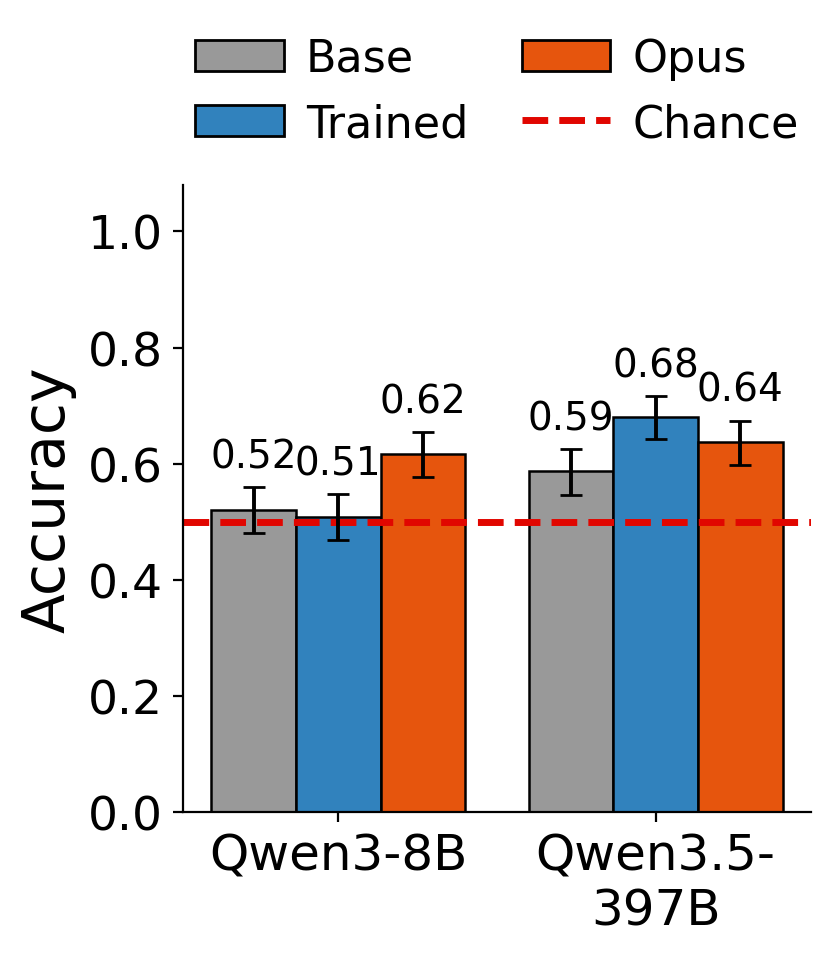
\includegraphics[width=.5\linewidth]{../papers/translations/chive/figures/self_explanation_hint_pooled_accuracy.png}
\caption{开放解释训练在397B暗示设置泛化, 8B不泛化. 问解释答案, 判断是否归因注入线索, 汇总迎合与MMLU. Opus对目标记录回答同问题第三人称. 仅训练397B优于基础并达Opus. 图例: Base＝基础, Trained＝训练, Opus reference＝参照; Accuracy＝准确率.}\label{chive-fig:hint_selfexpl}
\end{figure}
\begin{table}[ht]\centering
\begin{tabular}{llrrrr}\toprule
 & & \multicolumn{2}{c}{迎合} & \multicolumn{2}{c}{MMLU}\\
模型 & 分支 & FPR & TPR & FPR & TPR\\\midrule
Qwen3-8B & 基础 & .01 & .01 & .01 & .09\\
 & 训练 & .82 & .84 & .58 & .59\\
 & Opus参照 & 1.00 & 1.00 & .43 & .90\\\midrule
Qwen3.5-397B-A17B & 基础 & .00 & .00 & .03 & .38\\
 & 训练 & .31 & .61 & .29 & .70\\
 & Opus参照 & 1.00 & 1.00 & .36 & .91\\\bottomrule
\end{tabular}
\caption{开放自我解释的各暗示设置FPR/TPR, 每项150正、150负. 两率约0意味着从不归因暗示（基础模型）, 两率约1意味着总归因（Opus迎合）.}\label{chive-tab:selfexpl_hint_fpr}
\end{table}

\subsection*{E.3 留出调查的反事实可模拟性}\paperlabel{E.3}{chive-app:selfexpl_simulatability}
用反事实可模拟性评价开放解释: 是否帮助观察者预测输入反事实变体的输出\cite{chive-chen2023modelsexplainthemselvescounterfactual}. 已用于事后解释\cite{chive-chen2023modelsexplainthemselvescounterfactual,chive-mayne2026positivecasefaithfulnessllm}与思维链推理\cite{chive-hase2026counterfactualsimulationtrainingchainofthought}. 忠实解释应告知什么会改变行为. 模拟器得到记录加目标解释, 预测与正文相同二元主张, 对比同模拟器仅记录.

\textbf{训练不一致改善可模拟性.} 五模拟器从Gemma-3-12B到Opus4.8, 两目标的基础解释均无增益（图 \ref{chive-fig:heldout_selfexpl}、\ref{chive-fig:selfexpl_397b}）. 训练解释帮助弱模拟器、损害强模拟器. 训练产生自信具体而常错的反事实（暗示评价差可见）, 误导模拟器. 与Mayne等正面案例不同\cite{chive-mayne2026positivecasefaithfulnessllm}, 也许任务分布不同: 他们研究结构化表格分类决策解释, 我们研究开放提示的异常或错误.
\begin{figure}[ht]\centering
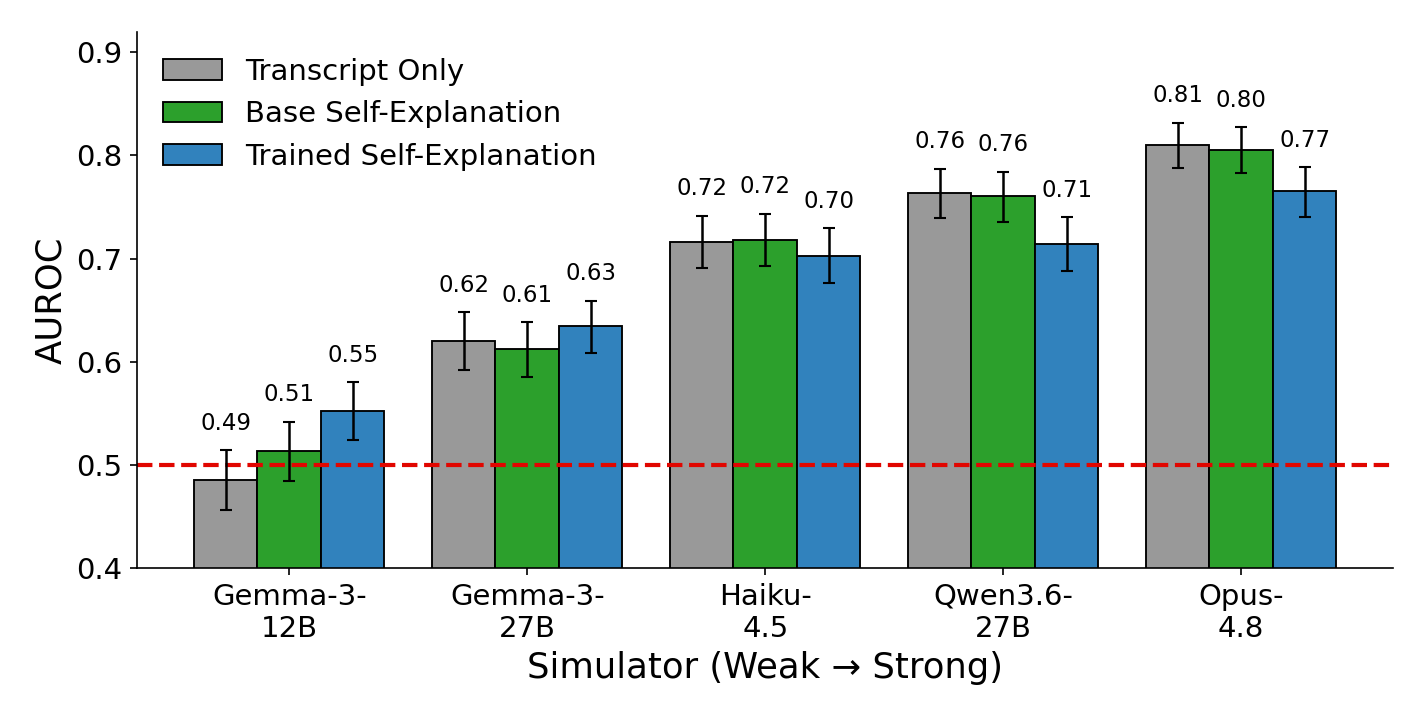
\includegraphics[width=.95\linewidth]{../papers/translations/chive/figures/figure_selfexpl_by_target.png}
\caption{开放解释训练帮助弱、损害强模拟器（Qwen3-8B）. 各模拟器看记录加自身解释预测留出主张, 对比仅记录. 基础解释无增益, 训练解释帮助最弱者, 却一致损害最强者; 它们能力足够, 会被自信具体常错解释误导. 图中文字: Simulator＝模拟器, Transcript only＝仅记录, Base explanation＝基础解释, Trained explanation＝训练解释, AUROC/uplift＝面积/增益; Simulator (Weak → Strong)＝模拟器（由弱至强）.}\label{chive-fig:heldout_selfexpl}
\end{figure}
\begin{figure}[ht]\centering
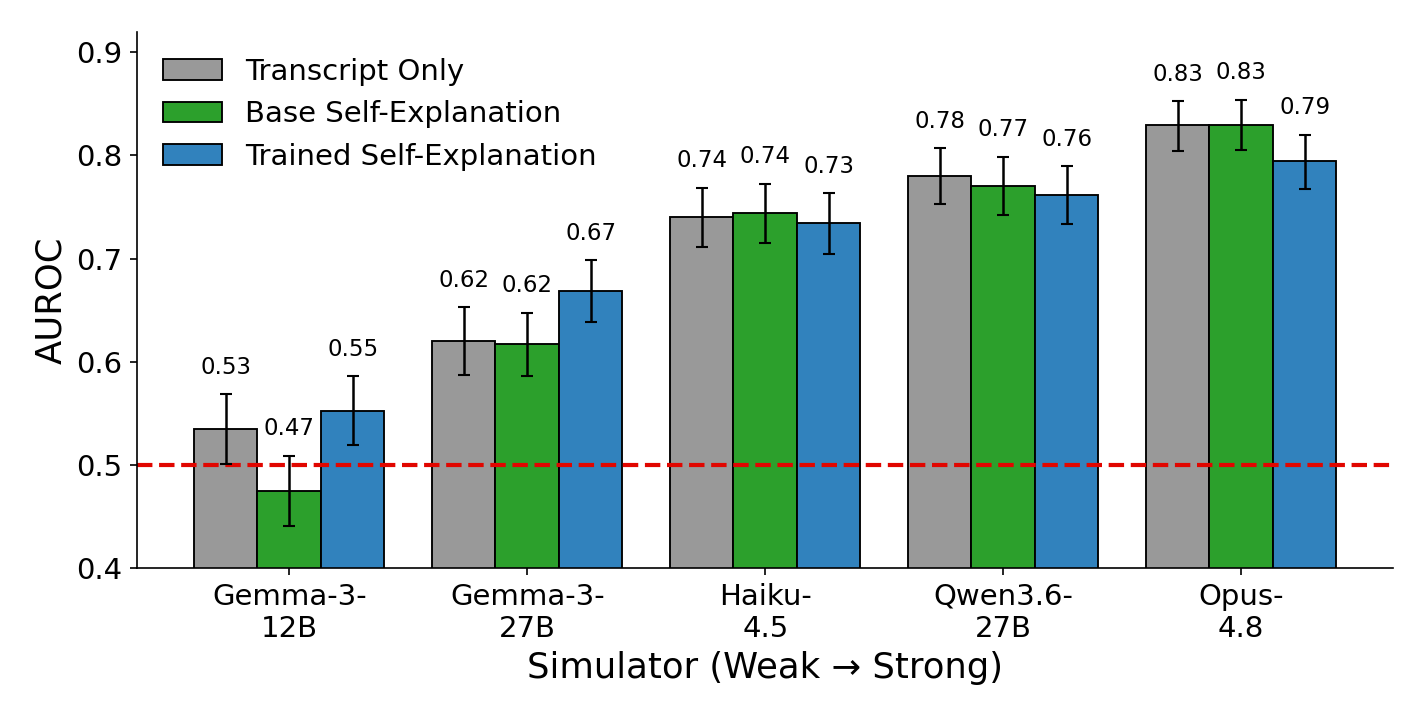
\includegraphics[width=.95\linewidth]{../papers/translations/chive/figures/figure_selfexpl_397b.png}
\caption{Qwen3.5-397B-A17B反事实可模拟性（WildChat）. 如8B一样, 各模拟器看记录与解释预测, 对比仅记录. 基础无增益; 训练帮助最弱、损害最强. 图例: Transcript only＝仅记录, Base explanation＝基础解释, Trained explanation＝训练解释; 纵轴为AUROC, 横轴模拟器型号（由弱至强）.}\label{chive-fig:selfexpl_397b}
\end{figure}

\subsection*{E.4 讨论: 怎样理解混合结果}\paperlabel{E.4}{chive-app:selfexpl_discussion}
采用这两评价因已有先前工作: 暗示归因来自思维链忠实性文献\cite{chive-turpin2023languagemodelsdontsay}, 反事实可模拟性来自Chen等.\cite{chive-chen2023modelsexplainthemselvescounterfactual}

两指标也许低估所学. 暗示是大分布偏移: 训练记录长, 多合理驱动因素; 暗示记录短、单个显著植入线索. 可模拟性依赖模拟器能力. 记录常长且杂乱, 解释通常不精确回答某特定反事实, 弱模拟器可能利用不了大体正确解释. 最强者仅记录已能很好预测, 需训练大改善才能带来增益.

尝试LLM直接判解释正确, 但不可靠, 因解释常提接近相关实验但不完全匹配的东西. 基础模型解释更长、有更多独立猜测, 会抬高召回式评分. 所以过滤为原因是单无歧义触发因素的调查, 如产生行为的特定短语, 评分是否提到它. 所有开放解释训练模型都一致改善. 但评价有循环性: 训练和评价同LLM流程生成, 仅作初步证据. 为多候选原因的杂乱记录开发干净指标, 是值得做的后续工作.
